\documentclass{article}
\usepackage[utf8]{inputenc}
\usepackage[lmargin=3cm,tmargin=3cm,rmargin=2cm,bmargin=2cm]{geometry}
\usepackage[onehalfspacing]{setspace}
\usepackage[T1]{fontenc}
\usepackage[brazil]{babel}


\usepackage{multicol}
\setlength{\columnsep}{-4cm}

\usepackage{graphicx}
\graphicspath{ {./plots/} }

\title{Análise de Mercado do Mato Grosso \\
 Soja e Fertilizantes}
\author{Luiz Eduardo de Lima}
\date{}

\begin{document}

\maketitle

\section*{Visão Geral}
Em 2021 o estado do Mato Grosso foi o maior produtor de soja do Brasil com $35,34$ milhões de toneladas produzidas representando $20,3\%$ da produção brasileira total.
\begin{center}
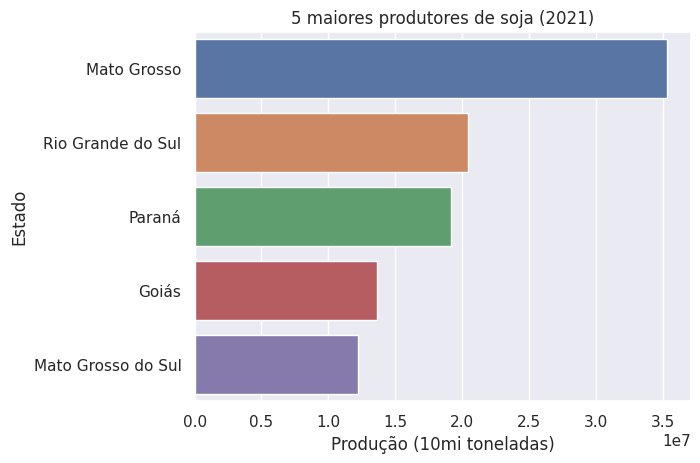
\includegraphics[scale=0.6]{top5_prod_soja_br.png}
\end{center}
Olhando para os últimos anos o Mato Grosso sempre apresentou crescimento na produção de soja e no valor total da produção. No ano de 2021 há um descasamento entre o volume produzido e o valor, isso ocorre por conta do aumento de um \textbf{choque negativo de oferta} por conta dos efeitos da pandemia da Covid que travaram as cadeias produtivas levando à uma alta de preços.
\\~\\
O primeiro caso de Covid-19 reportado em Wuhan foi em dezembro de 2019, porém estudos apontam que os primeiro casos provavelmente datam de novembro\footnote{fonte: https://journals.plos.org/plospathogens/article?id=10.1371/journal.ppat.1009620}, além disso, sabemos que a China é uma autocracia e não podemos confiar muito nos dados divulgados.
\\~\\
Outro fator importante para o mercado de soja é o agravamento da Guerra Russo-Ucraniana com a Batalha de Kiev iniciada em fevereiro de 2022. Na data atual (14/01/2022) o Instituto Brasileiro de Geografia e Estatística (IBGE) ainda não disponibilizou os dados concretizados da produção de 2022 para um análise mais adequada de como o conflito afeta o mercado de soja brasileiro.
\begin{center}
\includegraphics[scale=0.6]{soja_mt.png}
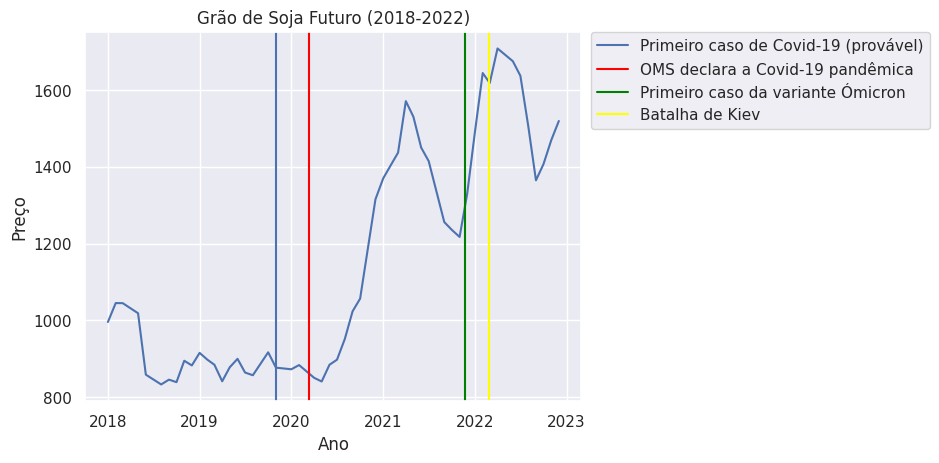
\includegraphics[scale=0.6]{soja_futuro.png}
\end{center}
\section*{O Mercado no Mato Grosso}
No cenária hipótico da abertura de um empresa fertilizantes no Mato Grosso precisamos responder algumas perguntas: 1) "qual o objetivo da empresa?", 2)"qual o indicador correto?", e, 3) "como é o mercado local?".
\\~\\
A primeira pergunta depende do estágio em que a empresa encontra-se, se estamos falando de um empresa nova devemos focar no \textit{marketshare} dela, se falamos de uma filial de uma companhia já consolidada no mercado o foco deve ser na geração de caixa.
\\~\\
Assumindo que seja o primeiro caso, considerando o marketshare precisamos levar em conta o volume produzido pela cidade. As 10 cidades mato-grossences que mais produziram soja em 2021 foram:
\\
\begin{multicols}{2}
\begin{tabular}[10pt]{|l | r|}
\hline
            Município &     \parbox[t]{2cm}{Volume \\ (Toneladas)} \\ \hline
              Sorriso &                        		 2.010.960 \\
           Nova Mutum &                         1.337.280 \\
              Sapezal &                         1.319.731 \\
           Diamantino &                         1.315.239 \\
   C. Novo do Parecis &                         1.304.958 \\
         Nova Ubiratã &                         1.301.915 \\
            Querência &                         1.298.304 \\
             Canarana &                         1.053.000 \\
   		  P. do Leste &                           939.600 \\
            Brasnorte &                           851.453 \\ \hline
	            TOTAL &                        12.732.440 \\ \hline
\end{tabular}

\columnbreak
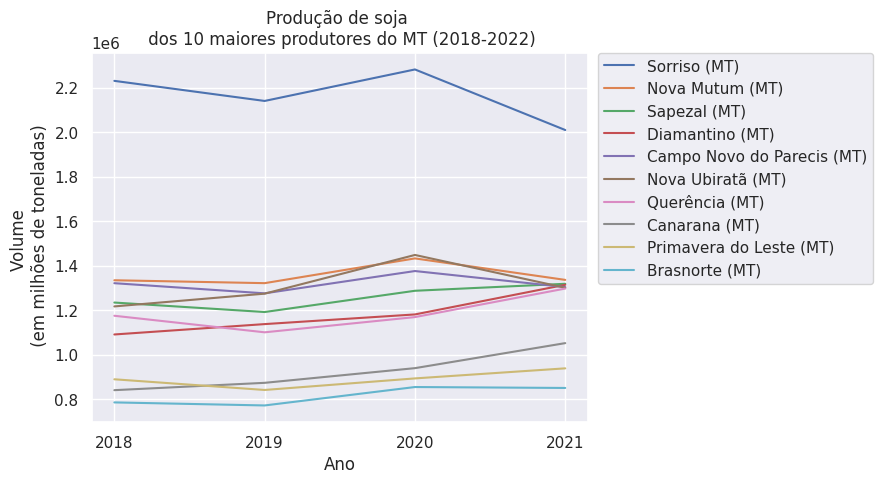
\includegraphics[scale=0.5]{top10_soja_mt_hist.png}
\end{multicols}
\subsection*{Despesas com Fertilizantes}
Nos dados da Companhia Nacional de Abastecimento (Conab) não constam os dados para todos os 10 municípios em questão, apenas de Sorriso, Campo Novo do Parecis e Primavera do Leste.

\begin{center}
\textbf{Despesa com fertilizantes por Hectare (em reais)}
\begin{tabular}[10pt]{|l|rrrrrrr|}
\hline
Município &    2018 &    2019 &    2020 &     2021 &     2022 &  \parbox[c]{1.5cm}{Média \\ Municipal} &  \parbox[c]{1.5cm}{Média \\ Var. (\%)} \\
\hline
Sorriso                &  702.20 &  892.50 &  913.50 &  1320.76 &  2565.44 &    1278.880 &           33.07 \\
Primavera do Leste     &  795.80 &  957.06 &  987.05 &  1046.69 &  2658.01 &    1288.922 &           26.80 \\
Campo Novo do Parecis  &  691.63 &  903.60 &  766.22 &   910.30 &  2244.92 &    1103.334 &           24.92 \\ \hline
Média Anual            &  730.00 &  918.00 &  889.00 &  1093.00 &  2489.00 &    1223.800 &           28.19 \\
Desvio Padrão          &   41.00 &   24.00 &   80.00 &   148.00 &   153.00 &      89.200 &           34.63 \\
Desvio Padrão Rel. (\%) &    6.00 &    3.00 &    9.00 &    14.00 &     6.00 &       7.600 &          -20.00 \\
\hline
\end{tabular}
\end{center}
Apesar de termos poucos dados vemos que o desvio padrão relativo é baixo, sempre abaixo de 10\% com excessão de 2021, essa variação maior pode ocorrer porque alguns municípios tinham estoques maiores ou outros fatores. Por conta disso vamos assumir que os outros minucípios consumam a média  $\pm$ um desvio padrão por hectare com fertilizantes.

\section*{Projeções}
Projetando a produção de acordo com a média da variação temos que em 2023 os municípios do Mato Grosso gastarão entre R\$3.400,00 e R\$ 2.950,00. Pensando nisso, precisamos elencar os municípios por sua área destinada ao plantio de soja:
\begin{center}
\textbf{Área destinada ao plantio de soja em hectares}
\begin{tabular}{|l|llllr|}
\hline
Município &      2018 &      2019 &      2020 &      2021 & \parbox[c]{1.5cm}{Média\\ Var. (\%)} \\
\hline
Canarana (MT)              & 255.000 & 265.000 & 285.000 & 300.000 &           3.75 \\
Diamantino (MT)            & 337.000 & 345.000 & 345.600 & 384.605 &           3.09 \\
Brasnorte (MT)             & 226.000 & 230.000 & 230.000 & 248.963 &           2.31 \\
Nova Ubiratã (MT)          & 350.000 & 366.482 & 396.000 & 382.677 &           2.13 \\
Querência (MT)             & 350.000 & 360.000 & 360.000 & 368.000 &           1.22 \\
Sapezal (MT)               & 355.000 & 355.000 & 352.000 & 366.592 &           0.79 \\
Sorriso (MT)               & 600.000 & 605.000 & 590.000 & 605.000 &           0.21 \\
Nova Mutum (MT)            & 400.000 & 402.000 & 395.000 & 398.000 &          -0.13 \\
Campo Novo do Parecis (MT) & 380.000 & 380.000 & 389.000 & 371.711 &          -0.56 \\
Primavera do Leste (MT)    & 280.000 & 270.000 & 257.000 & 270.000 &          -0.93 \\
\hline
\end{tabular}
\end{center}
\begin{multicols}{2}
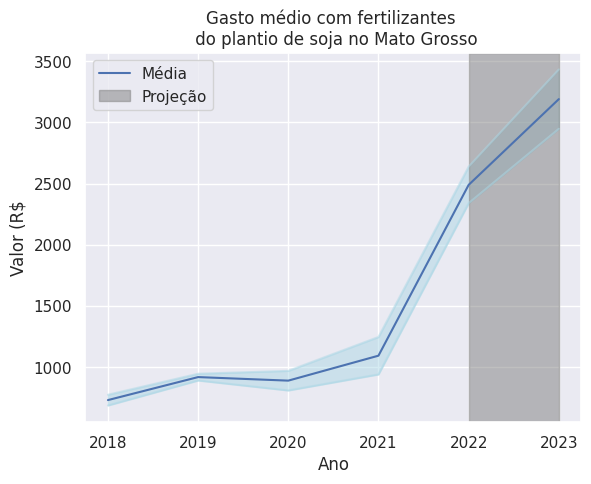
\includegraphics[scale=0.4]{proj_fert.png}
\columnbreak
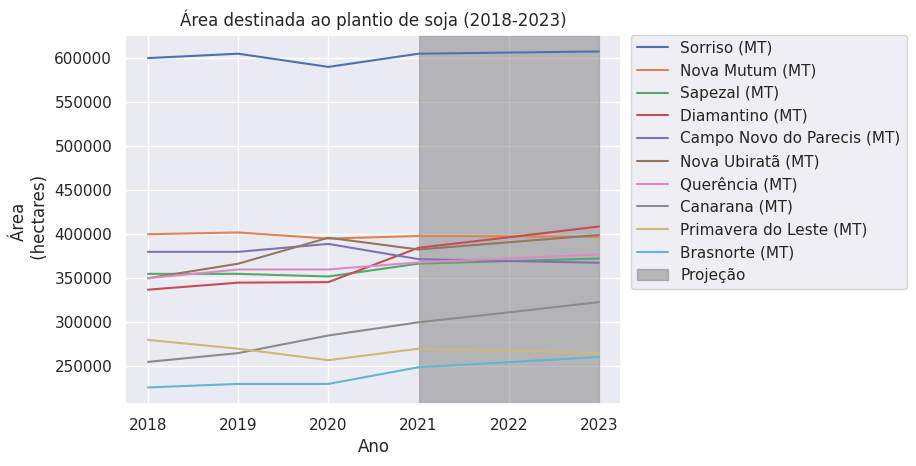
\includegraphics[scale=0.4]{area_plantio_proj.png}
\end{multicols}
\section*{Conclusões}
Considerando os dados disponíveis e as projeções a nova loja de revenda de fertilizantes é Nova Mutum. Apesar de apresentar uma queda na área destinada ao plantio de soja ainda é a segunda maior produtora de soja do estado.
\\~\\
Outro fator que justifica essa escolha é a localização da cidade, ficando apenas a 160km de distância de Sorriso, que é a maior produtora do estado, 130km de Diamantino, a segunda cidades onde a área destina ao plantio mais cresceu, 220km de Campo Novo do Parecis, a sexta maior produtora de soja e a 180km de Nova Ubiratã, sétima maior produtora de soja. 
\end{document}